\chapter{Discussion} \label{ch:discussion}

\section{Threshold calibration}
Different localization methods exhibit different localization performance distributions, as illustrated in Fig. \ref{fig:boxacc_resnet50_imagenet}. Here we show the box accuracy (BoxAccV2 as defined in equation \ref{eq:boxaccv2}) using different localization methods for the ResNet-50 network on the ImageNet validation dataset. We use a BoxAcc plot to illustrate box accuracy in function of the score map threshold. Fig. \ref{fig:boxacc_resnet50_imagenet} clearly shows that each localization method has a different BoxAcc distribution. Fixing the score map threshold at a single pre-defined value, could lead to increased performance of some methods and to decreased performance for others. 

The threshold-independent localization metric MaxBoxAccV3 recall (MaxBoxAccV3 in short) is then the maximum value of the BoxAcc metric in the plot. The optimal score map threshold is the score map threshold for the maximum box accuracy. We observe that the localization methods have different optimal score map thresholds, but the MaxBoxAccV3 values are not significantly different. This provides an explanation of the limited differences between localization methods for MaxBoxAccV3 recall as observed in Table \ref{tab:metrics_resnet50_imagenet}.

\begin{figure}[ht]
    \begin{center}       
    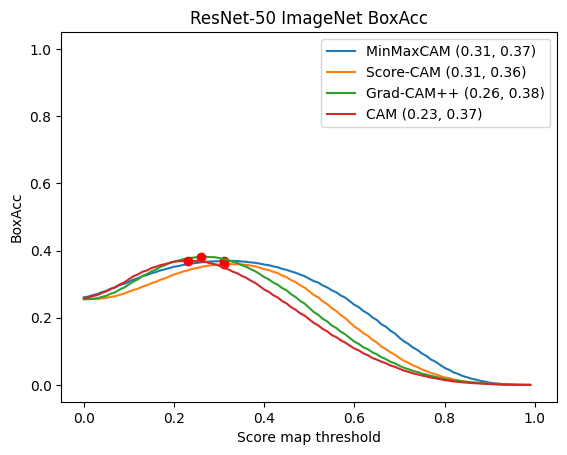
\includegraphics[width=0.7\textwidth]{fig_boxacc_resnet50_imagenet.png}
    \caption[BoxAcc (IoU 50)for ResNet-50 on ImageNet]{Performance at varying operating thresholds. BoxAcc($\tau$) versus score map threshold $\tau$ at IoU threshold 50 for ResNet-50 on ImageNet.}
    \caption*{Source: Author}
    \label{fig:boxacc_resnet50_imagenet}
    \end{center}
\end{figure}

\section{Classification versus localization accuracy}
When comparing classification accuracy with localization accuracy (MaxBoxAccV3 recall) during training, we observed that there is a correlation between both metrics. Fig. \ref{fig:loc_vs_acc_vgg16_gap_cam_synthetic} illustrates that classification accuracy and CAM localization accuracy (MaxBoxAccV3 recall) for VGG16-GAP on each of the validation synthetic datasets, improve during the early epochs of training, until both metrics start converging.

A question is then which checkpoint during training is suitable for localization evaluation? Choe \textit{et al.} \cite{choe2020evaluating} argue that in many cases, the best localization performances are achieved before convergence, that at early epochs, the localization can fluctuate a lot and thus, peak performance is noise rather than real performance. Fig. \ref{fig:loc_vs_acc_resnet50_cam_d1b} illustrates such case for the CAM localization method on ResNet-50 for the d1b synthetic dataset. We clearly see that the maximum value for MaxBoxAccV3 is reached during the early training epochs, and drops around epoch 10 before converging.

To avoid measuring noise, we use an early stop criterion that ends model training when classification accuracy has not improved the best accuracy for five consecutive training epochs. We then take as localization accuracy the value computed at the last epoch on the validation dataset.

\begin{figure}[ht]
\begin{center}
    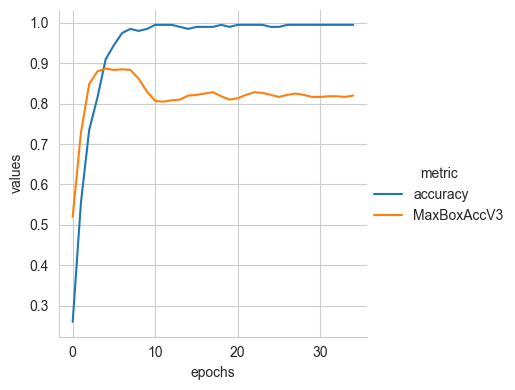
\includegraphics[width=0.6\textwidth]{images/fig_loc_vs_acc_resnet50_cam_d1b.png}
    \caption[Classification versus CAM localization accuracy on ResNet-50 for d1b dataset]{Classification versus CAM localization accuracy on ResNet-50 for d1b dataset.}
    \caption*{Source: Author}
    \label{fig:loc_vs_acc_resnet50_cam_d1b}
\end{center}
\end{figure}

\section{Iterative localization}
The results of the iterative localization experiments in section \ref{sec:exp_loc_improvements} showed that localization accuracy can be improved using the iterative approach on all localization metrics. Depending on the mask strategy, merge strategy and chosen stop criterion recall can be improved substantially. In most cases, recall improvement comes at the cost of precision loss when compared with the baseline.

The two parameters that are most important for improving recall, are the merge strategy and the iteration stop criterion. The mask strategy has smaller impact on the recall. 

For the synthetic datasets with multiple object instances and in the ImageNet dataset, the experiments using the 'add' merge strategy and iteration stop threshold 1.0 have the most substantial gain in recall but at a large impact on precision. It is easy to see that in this scenario each iteration potentially adding more bounding boxes, potentially increases matches  or mismatches between predicted and ground truth bounding boxes, hence increasing recall in the former and decreasing precision in the latter case.

The experiments with the large and diverse ImageNet dataset shows that is quite some room for improving localization accuracy. However, the current iterative approach stills suffers from substantial loss in precision. In our current approach we use bounding boxes predicted in previous iterations as image masks to predict new boxes. As future work it would be interesting to evaluate using the more fine-grained score map as an image mask for improving precision.